% !Mode:: "TeX:UTF-8"

\chapter{基于深度学习的声学建模}\label{intro_dl}


深度学习在语音识别中的引入,替代了经典HMM-GMM系统中采用GMM对状态概率密度进行建模的方法,
使用深度神经网络对状态的概率分布进行建模,称之为基于HMM-DL(HMM-Deep Learning)的语音识别系统。

本章介绍深度学习的基本原理和在语音识别中的基本应用。以下介绍几种常见的神经网络结构全接连的神经网络DNN、
卷积神经网络CNN、循环神经网络RNN等深度学习网络的基本结构;
研究这些深度学习网络在语音识别这个特定任务中的使用方式,改进和组合使用(CLDNN)等;
最后本章给出这几种深度学习方法的相关实验。

\section{HMM-DL系统}\label{section:hmmdl}

在经典HMM-GMM的语音识别系统中,为每个状态建立一个GMM模型来描述其概率分布,
在识别时,通过各自状态的GMM可以直接计算$t$时刻的观测$o_t$在状态$s_i$上的概率
$p(o_t|s_i)$,$p(o_t|s_i)$HMM系统识别时必须的依赖。

深度学习引入语音识别后,使用深度神经网络来替代GMM对每个状态进行建模,
在深度神经网络中,这是一个典型的分类任务,即当新的一帧语音到来时,
通过深度神经网络计算其在每个状态上的概率。
与GMM系统为每个状态建立独立的GMM模型不同,深度神经网络本身为紧凑模型,即所有状态共享一个模型。
通过深度神经网络直接计算出的是$p(s_i|o_t)$,而非$p(o_t|s_i)$,
这是基于GMM和神经网络对声学模型进行建模的一个本质上的不同。

通过贝叶斯公式有:
\begin{equation}
p(o_t|s_i) = \frac{p(s_i|o_t)p(o_t)}{p(s_i)}
\end{equation}
在识别的解码过程中,为防止概率连乘导致下溢,概率计算一般转到$log$域,取$log$有:
\begin{equation} \label{equation:hmmdnn}
\begin{array}{l}
\log{p(o_t|s_i)} = \mathop {\log{p(s_i|o_t)} + \log{p(o_t)} - \log{p(s_i)}} \\
\;\;\;\;\;\;\;\;\;\;\;\;\;\;\;\;\; = \mathop {\log{p(s_i|o_t)} - \log{p(s_i)}}
\end{array}
\end{equation}
其中$p(o_t)$为$o_t$发生的概率,对所有的状态相同,因此可以忽略。
$p(s_i)$为状态$s_i$出现的概率,称之为状态先验,一般可以通过对训练数据集作状态统计得到。
通过公式\ref{equation:hmmdnn},便可以计算得到$p(o_t|s_i)$,这是基于HMM-DL系统进行语音
识别的基本原理。
如图\ref{fig:hmmdnn}所示,原始语音信号经过特征提取,输入到神经网络,
计算当前信号在每个状态上的概率,然后结合该概率在HMM系统中进行语音识别解码。


\begin{figure}
\centering
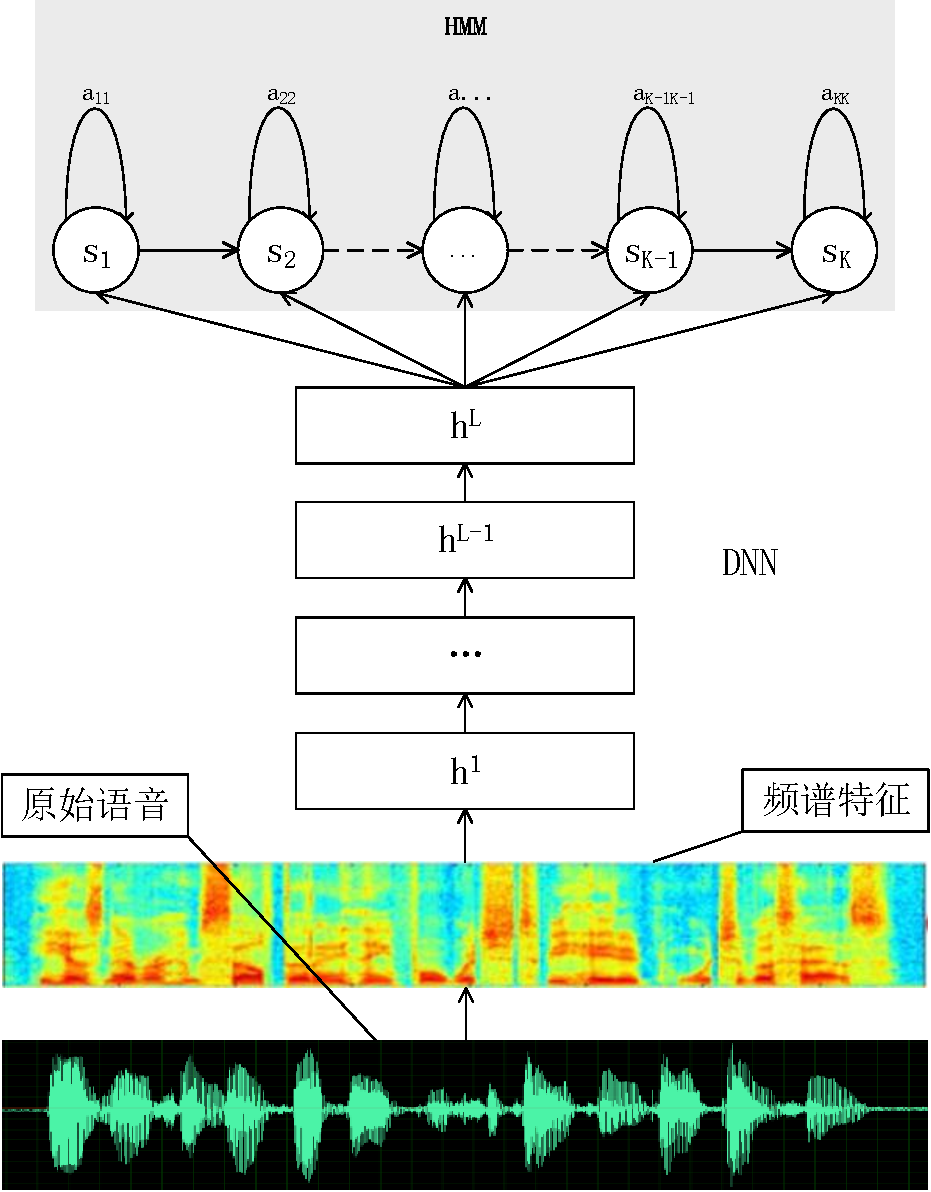
\includegraphics[width=0.6\textwidth]{figures/chapter3/hmmdnn-crop}
\caption{HMM-DL系统的基本原理}
\label{fig:hmmdnn}
\end{figure}


\section{全连接神经网络DNN}

深度神经网络DNN\ucite{bengio2012practical}(Deep Neural Network)是有多个(一般均大于2层)隐层的传统的多层感知机MLP(MultiLayer Perceptron)。
一个典型的神经网络由输入层;中间多个隐层和输出层组成。
如图\ref{fig:dnn}所示DNN,含有3个隐层,每个隐层有5个节点。
在一个$L+1$层的DNN中,我们定义输入层为第$0$层,输出层为第$L$层。

\begin{figure}
\centering
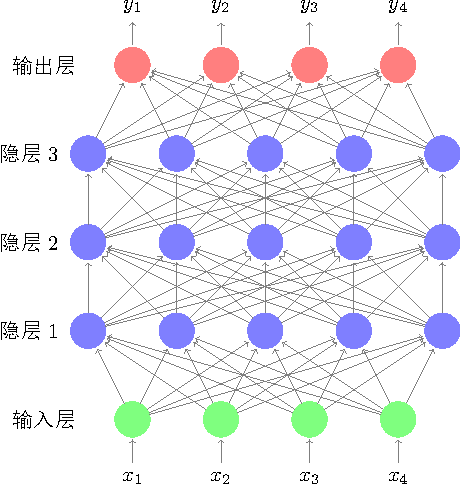
\includegraphics[width=0.5\textwidth]{figures/chapter3/dnn-crop}
\caption{DNN示例(该DNN由输入层、3个隐层和输出层组成)}
\label{fig:dnn}
\end{figure}

对于任意隐层$l$的任意节点$j$,有:
\[\begin{array}{l}
a_j^l = \sum\limits_{i = 1}^N {w_{ji}^l {x_i}^{l-1}+ b_j^l} \\
z_j^l = h(a_j^l)
\end{array}\]

其中,$i = 1,...,N$表示$l-1$层的节点数目,$a_j^l$表示第$l$层第$j$个节点的激励,
$a_j^l$经过激活函数$h(.)$作用得到$z_j^l$。
通常$h(.)$为非线性的、可导函数,
通过非线性函数增强神经网络的非线性映射能力,可导性则可以使神经网络通过梯度的方法行优化。

\subsection{激活函数}

在深度神经网络的实际应用中,最常用的激活函数是$sigmoid$函数:
\begin{equation}
s(z) = \frac{1}{{1 + {e^{ - z}}}}
\end{equation}
或者$tanh$函数:
\begin{equation}
\tanh (z) = \frac{{{e^z} - {e^{ - z}}}}{{{e^z} + {e^{ - z}}}}
\end{equation}
$sigmoid$函数将输入通过非线性函数映射到空间$(0,1)$;$tanh$函数的值域空间为$(-1,1)$,
其映射空间具有对称性。$ReLU$\ucite{glorot2011deep}是近年深度学习技术流行之后,又一个非常有效的激活函数:
\begin{equation} \label{equation:relu}
{\mathop{\rm Re}\nolimits} LU(z) = \max (0,z)
\end{equation}
$ReLU$激活函数预测具有稀疏性,这中预测特性提高了网络的泛化能力;另一方面,
如式\ref{equation:relu},$ReLU$的梯度形式简单,非0即1,有效的缓解了深度神经网络
训练中的梯度弥散问题;而且$ReLU$激活函数的计算更加简单,速度更快。
三种激活函数如图\ref{fig:activation}所示。

\begin{figure}
\centering
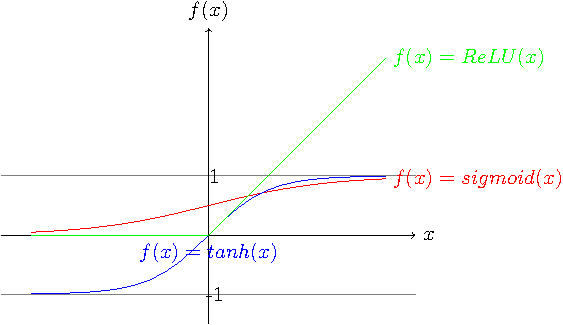
\includegraphics[width=0.6\textwidth]{figures/chapter3/activation-crop}
\caption{激活函数$sigmoid$,$tanh$,$ReLU$对比}
\label{fig:activation}
\end{figure}

激活函数的选择和深度神经网络密切相关,因此设计更好的激活函数也成为当下深度学习研究的热点之一,
最近的实验\ucite{zhang2014improving, zhang2015parameterised}表明,经过精心设计的激活函数能够
在一定程度上提高深度神经网络的性能。

\subsection{DNN训练}

DNN的训练即在损失函数确定后,使用误差方向传播BP(Back Propagation)算法计算参数梯度,
使用随机梯度下降SGD(Stochastic Gradient Descent)对模型中的参数进行更新。

一般来说,对于回归任务,使用最小均方误差MSE(Mean Suqare Error)损失函数:
\begin{equation}
E({\rm{w}}) = \frac{1}{2}\sum\limits_{n = 1}^N {\{ {y_n}}  - {t_n}{\} ^2}
\end{equation}
其中$y_n$为网络输出,$t_n$为标注,$N$为样本总数。

对于分类任务,首先应用$softmax$函数:
\begin{equation}
{y_k} = \frac{{\exp ({a_k})}}{{\sum\limits_j {\exp ({a_{\rm{j}}})} }}
\end{equation}
计算在每个类别上的归一化后的概率,然后使用交叉熵CE(Cross Entropy)准则计算损失:
\begin{equation}
E(w) =  - \sum\limits_{n = 1}^N {\sum\limits_{k = 1}^K {{t_{kn}}\ln {y_k}} }
\end{equation}

根据\ref{section:hmmdl},基于深度神经网络的声学建模为典型的分类任务,
在输出层使用$softmax$函数做概率归一,使用交叉熵作为损失函数。

\section{卷积神经网络CNN}

CNN最早应用在图像领域,在基础DNN的结构上,CNN引进了局部滤波器,池化层和权值共享三个新思想。
深度学习在语音识别领域获得成功后,研究人员开始探索CNN在语音识别任务上的应用。

语音信号在频域上具有一定的局部特性,不同的音素在不同的局部频带上能量比较集中。
例如,非静音的音素在不同频带上有一定的共振峰。
在这些频带上应用局部滤波器或许能够提供对这些局部特征结构的更有效的表示,
这个特点是CNN能够应用在识别任务上的基础。

在语音识别中,CNN中使用卷积层能够对局部频域特征建模。
将输入语音信号分频带规整好之后,卷积层中每个卷积核的输入都为一定频段的语音信号。
假设输入信号$\textbf{x}$被分为$N$个频带$\textbf{x}= [\textbf{x}_1, \textbf{x}_2, ..., \textbf{x}_N]$,
其中向量$\textbf{x}_n$代表频段$n$。如图\ref{fig:cnn}所示,这个$\textbf{x}_n$可以包含原始频谱,一阶差分和二阶差分。
卷积层的激励被分为$K$个子带,每个频带包含$J$个滤波器的激励。
将每个子带的激励记作$\textbf{q}_k$ = $[q_{k,1}, q_{k,2}, ..., q_{k, J}]$,则有:
\begin{equation}
{{\rm{q}}_{k,j}} = h(\sum\limits_{n = 1}^{s - 1} {{\textbf{w}_{n,j}}\textbf{x}_{n{\rm{ + k}}}^T + {b_j})}
\end{equation}
其中,$h(.)$表示激活函数,$s$表示局部滤波器的宽度,$\textbf{w}_{n,j}$表示第$j$个滤波器的的第$n$维权重向量。


\begin{figure}
\centering
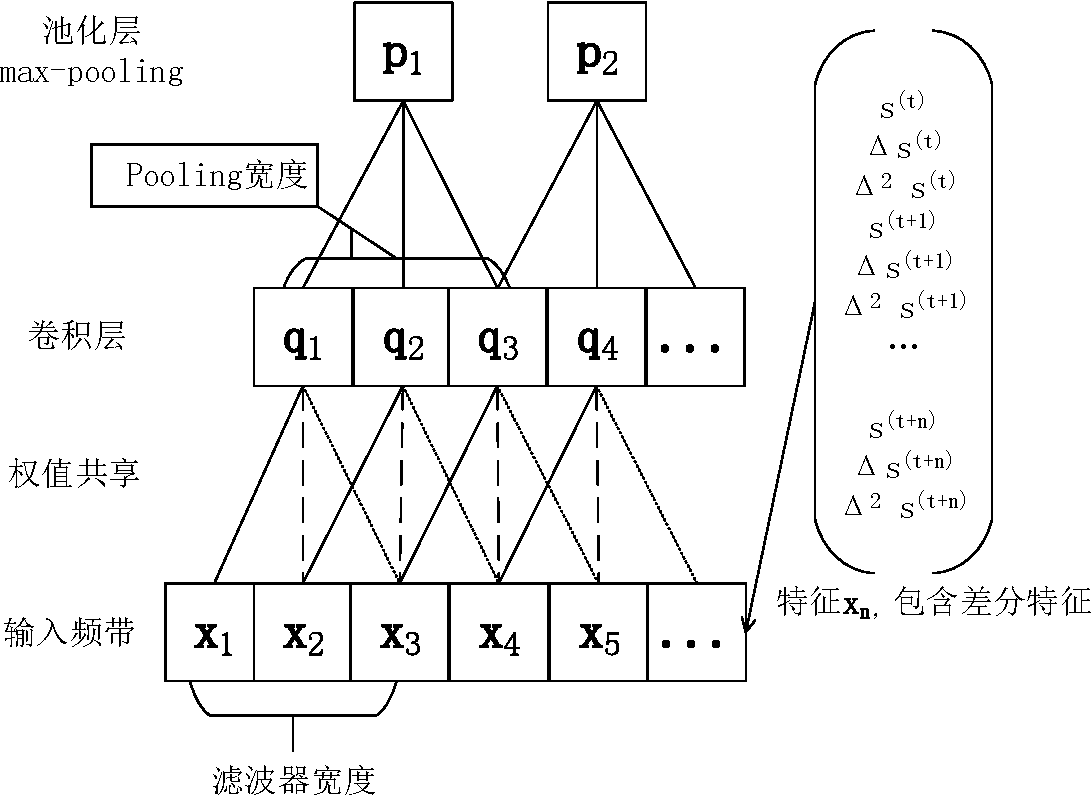
\includegraphics[width=0.6\textwidth]{figures/chapter3/cnn-crop}
\caption{CNN基本结构示意}
\label{fig:cnn}
\end{figure}

在CNN中,使用max-pooling(最大池化层)来保证局部不变性,max-pooling层一般位于卷积层之后,
作用在卷积层的激励输出上。max-pooling通过对局部激励取最大(max)操作,从而得到低分辨率的卷积层的输出,
这种表示更为抽象,更为鲁棒,随后作为高层神经网络的输入处理。
假设max-pooling操作共产生$M$个子带,将第$m$个子带的激励记作
$\textbf{p}_m$ = $[p_{m,1}, q_{m,2}, ..., q_{m, J}]$,则有:
\begin{equation}
{p_{m,j}} = \mathop {\max }\limits_{k = 1}^r ({q_{m \times n + k,j}})
\end{equation}
其中,$r$是pooling的大小,$n$是pooling的步长,一般小于$r$(这样允许临近的pooling操作可以有重叠),
图ref{fig:cnn}中,pooling的大小为3,步长为2.

基于CNN的语音识别网络如图\ref{fig:cnnasr}所示。如上分析,CNN的输入为频域特征,
Fbank(Filter bank)特征是目前最为常用的频谱特征。
神经网络的底层为一层或者多层的CNN,用作频谱特征的抽取,之后会连接普通的DNN神经网络。
基于CNN的语音识别也是目前识别领域的研究热点之一,
一种趋势是直接CNN直接对原始音频Raw进行建模\ucite{palaz2015convolutional, sainath2016factored},
另一种趋势应用已经在图像上应用获得成功的Deep CNN\ucite{yu2016deep, xiong2016microsoft, sercu2016very, saon2015ibm}的结构到语音识别任务中。


\begin{figure}
\centering
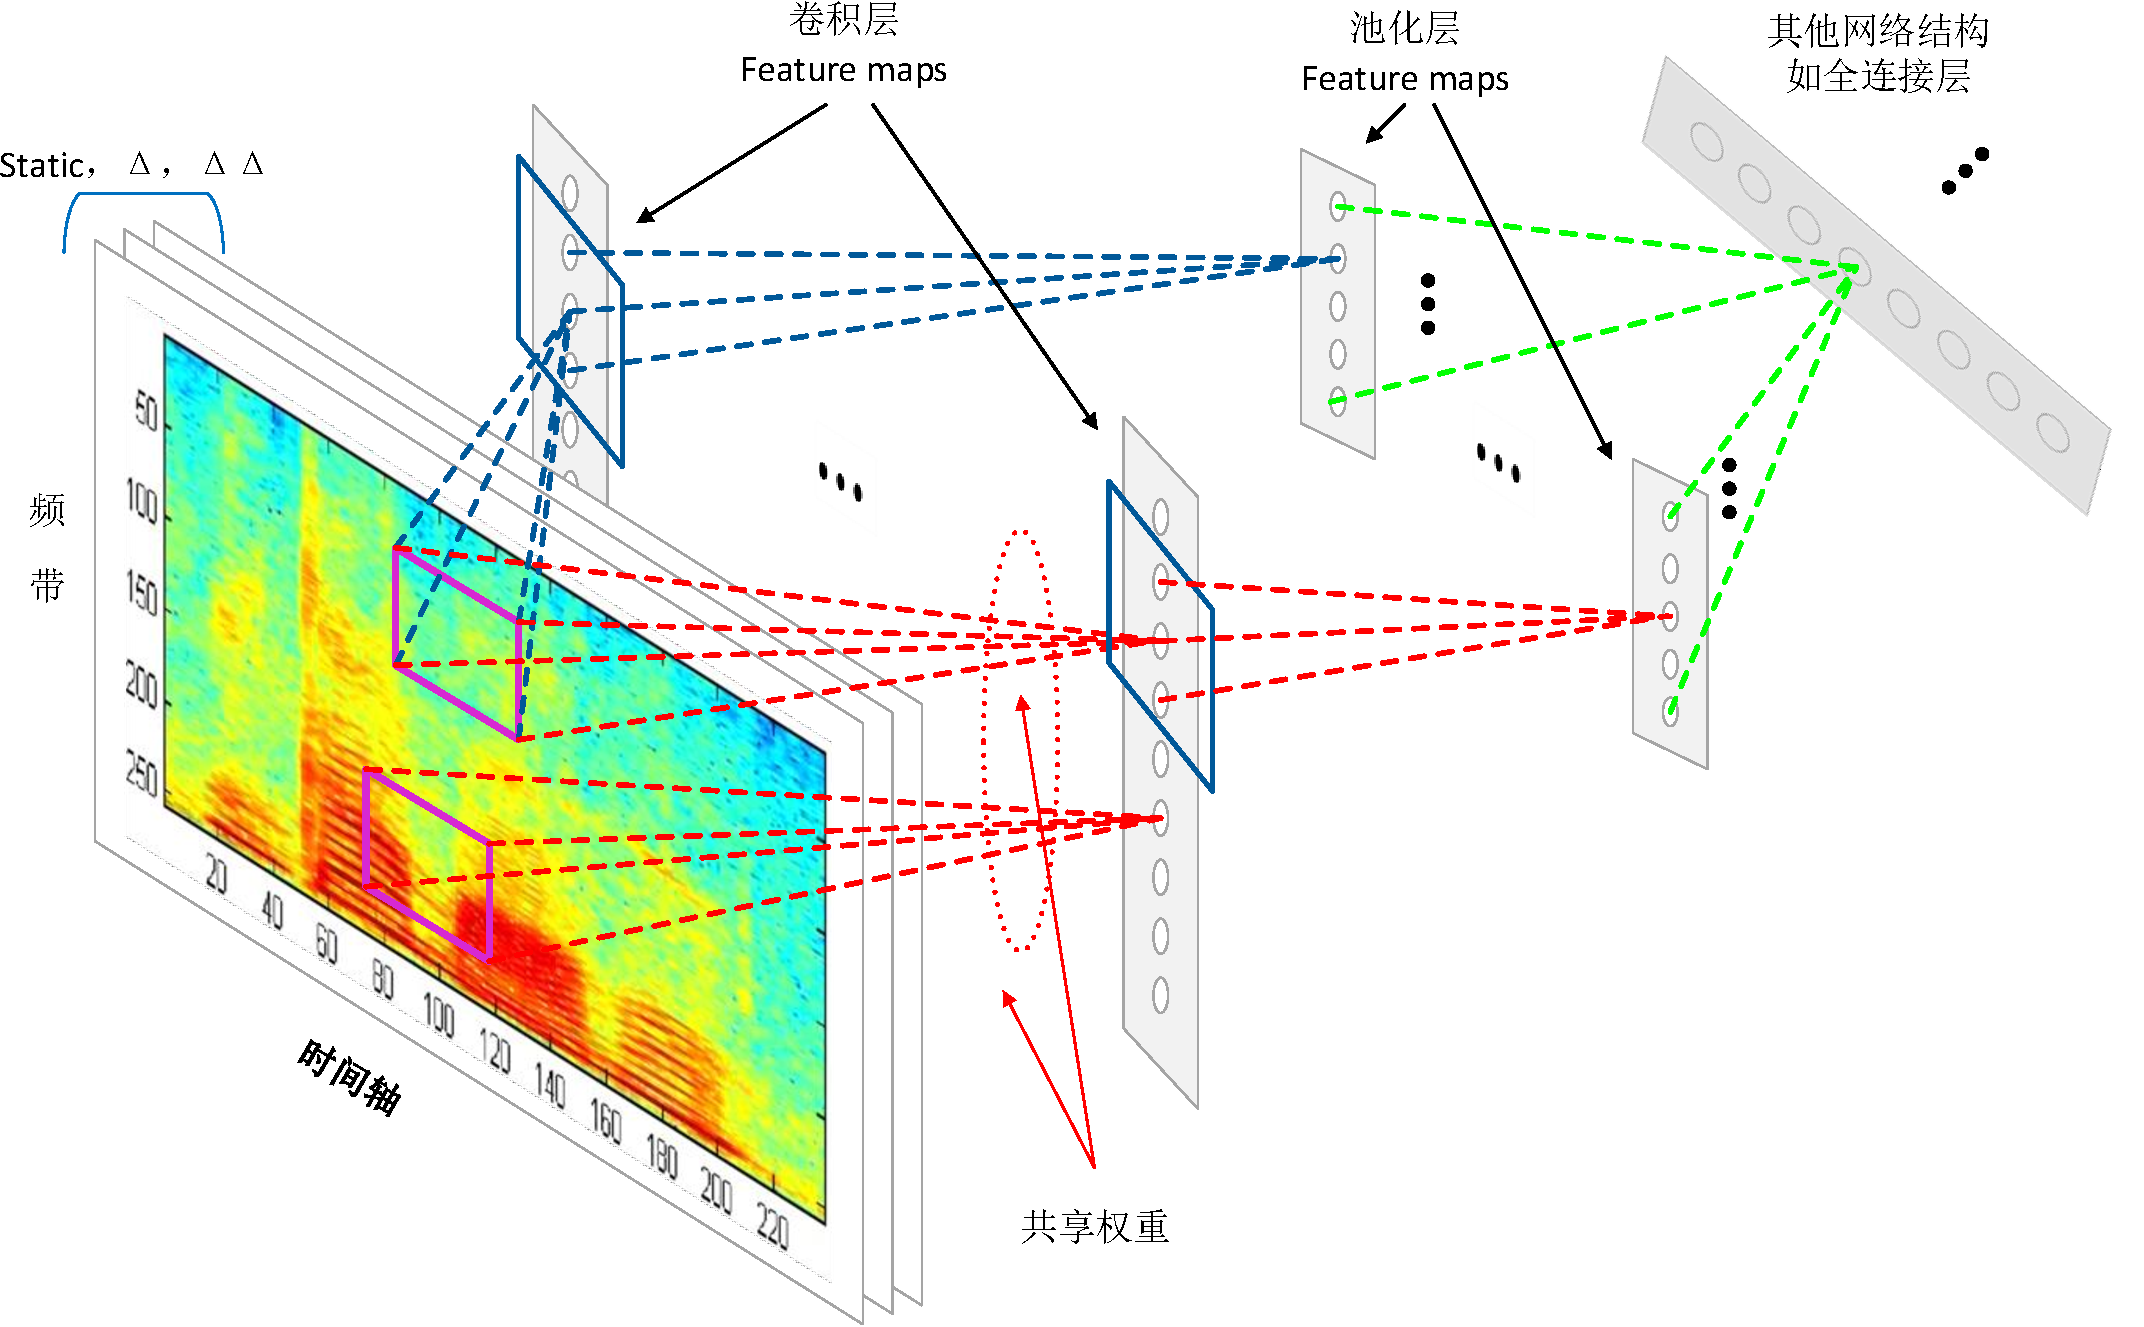
\includegraphics[width=0.8\textwidth]{figures/chapter3/cnnasr-crop}
\caption{基于CNN的声学模型}
\label{fig:cnnasr}
\end{figure}

\section{循环神经网络RNN}

\section{混合神经网络CLDNN}

\section{实验} 